\chapter{Konzeptionierung}
\label{chap:konzeption}
In diesem Kapitel wird auf Basis der Ergebnisse aus Kapitel \ref{chap:erwartungshaltung} ein System konzipiert, das als Teilsystem des Recommender System zur Mitarbeiterempfehlung dienen soll.
\section{Idee des Recommender System zur Mitarbeiterempfehlung}
Das zu unterstützende Recommender System zur Mitarbeiterempfehlung besteht aus mehreren Schritten.\\
\todo{meinen Teil eventuell farblich markieren}\\
\begin{figure}[H]
	\centering  
	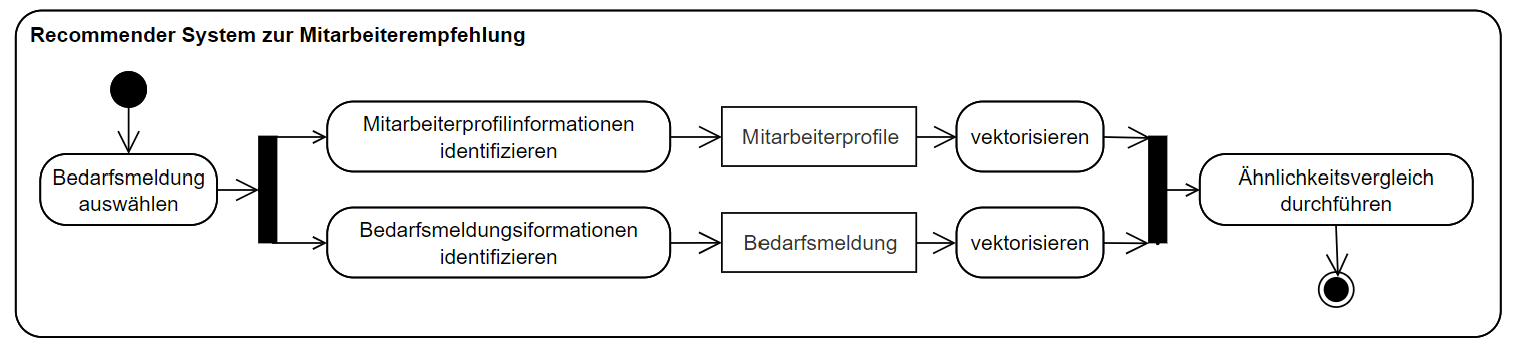
\includegraphics[width=\linewidth]{Abbildungen/recommendersystem.png}
	\caption{Abstrakte Darstellung des Recommender System zur Mitarbeiterempfehlung.}
	\label{fig:recommendersystem}
\end{figure}\mbox{} \\
Diese Schritte sind abstrakt als UML-Aktivitätsdiagramm in der Abbildung \ref{fig:recommendersystem} dargestellt. Nach Auswahl einer \emph{Bedarfsmeldung} wird diese einerseits auf die relevanten Informationen reduziert und strukturiert. Diesen Schritt gilt es in dieser Arbeit zu konzipieren, entwickeln und evaluieren. Neben diesem Schritt erfolgt eine Vorverarbeitung der Mitarbeiterprofile, bei dem die verfügbaren Informationen in eine vergleichbare Struktur wie die Bedarfsmeldung reduziert werden. Die strukturierte \emph{Bedarfsmeldung} und Mitarbeiterprofile werden vektorisiert und am Ende mit einer Vergleichsmetrik auf Ähnlichkeit geprüft. Die Komplexität der Vergleichsmetrik ist dabei skalierbar. So können verschiedene Aspekte, wie z.B. Verfügbarkeit, Skills, etc., Bestandteil des Ähnlichkeits-Scoring sein. Das Profil, bzw. die Profile mit der höchsten Ähnlichkeit zur \emph{Bedarfsmeldung} wird am Ende Empfohlen.
\paragraph{Recommender Systems Historie und aktueller Stand der Forschung}\label{sec:rechistory}\mbox{} \\
Auch wenn die Erstellung eines vollständigen Recommender Systems nicht Gegenstand der vorliegenden Ausarbeitung ist, stellt die Nutzung von Information Retrieval und Filtering ein entscheidener Schritt in Richtung eines funktionierenden Recommender Systems dar. Das Verständnis der Funktionsweise eines Recommender Systems sowie dessen Entwicklung in den vergangenen Jahren ist daher für das Verständnis des Teilbereichs dieser Thematik essentiell.\\

Recommender Systems existieren bereits seit vielen Jahren \cite{dong2022brief}. Im Jahr 1992 führten Belkin und Croft eine Analyse und einen Vergleich des Information Retrievals und Filtering durch \cite{dong2022brief}. Das Information Retrieval behandelt die grundlegende Technologie der Suchmaschine \cite{dong2022brief}. Das Recommender System basiert hauptsächlich auf der Technologie des Information Filtering. Im selben Jahr präsentierte Goldberg das Tapestry-System, das das erste System zur Informationsfilterung darstellt, das auf kollaboratives Filtern durch menschliche Bewertung basiert \cite{dong2022brief}. Die Mehrheit der frühen Empfehlungsmodelle basiert auf kollaborativer Empfehlungen, wobei K-Nearest-Neighbor (KNN)-Modelle eine besondere Rolle einnehmen. Diese Modelle prognostizieren die Nachbarn eines Zielnutzers, indem sie eine Ähnlichkeit zwischen den vorherigen Präferenzen und den Präferenzen der anderen Nutzer berechnen \cite{dong2022brief}. Die Studie von Goldberg inspirierte einige Forscher des Massachusetts Institute of Technology (MIT) und der University of Minnesota (UMN) dazu, einen Nachrichtenempfehlungsdienst mit dem Namen \emph{GroupLens} zu entwickeln. Die Hauptkomponente dieses Dienstes ist ein Modell zur kollaborativen Filterung zwischen Nutzern \cite{dong2022brief}. Das gleichnamige Forschungslabor kann somit als Pionier auf dem Gebiet der Recommender Systems bezeichnet werden. Die dort durchgeführten Forschungen bilden die Grundlage für nachfolgende Musik- und Video-Ähnlichkeitsempfehlungen \cite{dong2022brief}. \\

Recommender Systeme haben in den letzten Jahren verschiedene Definitionen erhalten. Eine dieser Definitionen wird in dem Artikel von Resnick und Varian (1997) sinngemäß so beschrieben, dass ein typisches Recommender System Empfehlungen durch Personen als Eingabe erhält, die das System dann zusammenschließt und an geeignete Empfänger weiterleitet \cite{burke2011recommender}. In einigen Fällen besteht die primäre Transformation in der Zusammenführung, in anderen Fällen liegt die Fähigkeit des Systems darin, gute Übereinstimmungen zwischen Empfehlungsgebern und Empfehlungsempfängern herzustellen \cite{burke2011recommender}. Empfehlungssysteme stellen ein Instrument zur Interaktion mit umfangreichen und vielschichtigen Informationen dar \cite{burke2011recommender}. Sie ermöglichen eine personalisierte Sicht auf diese Informationen, indem sie die für den Nutzer wahrscheinlich relevanten Inhalte aufbereiten \cite{burke2011recommender}. Besonders im Handelsverkehr im Internet sind Recommender Systeme ein häufiger Einsatzgebiet. Dabei werden Recommender Systeme als Werkzeuge zum Suchen und Filtern von Informationen verwendet, die dem Benutzer Vorschläge unterbreiten, die für ihn nützlich sein könnten \cite{burke2011recommender}. Sie sind in einer Vielzahl von Internetanwendungen weit verbreitet und helfen den Nutzern, bessere Entscheidungen bei der Suche nach Nachrichten, Musik, Urlaubsangeboten oder Geldanlagen zu treffen \cite{ricci2014recommender}. Eine spezifisches Recommender System konzentriert sich typischerweise auf eine Art von Themengebiet wie z. B. Filme oder Nachrichten \cite{ricci2014recommender}. Darüber hinaus sind sie zu einem entscheidenden Faktor in der Entscheidungsfindung von Organisationen geworden \cite{chartron2014general}. Unternehmen wie \emph{adesso} bauen immer weiter auf Recommender System unterstützte System auf, um Prozesse zu beschleunigen oder zu vereinfachen. Grundsätzlich können die Methoden in die Typen (i)\emph{collaborative Filtering-based} (kollaborative Empfehlungssysteme), (ii)\emph{content-based} (inhaltsbasierte Empfehlungssysteme), (iii)\emph{knowledge-based} (wissensbasiert Empfehlungssysteme) und (iv)\emph{hybrid} (hybride Empfehlungssysteme) unterteilt werden.\\

Jede Empfehlungsmethode hat ihre Vorteile und Grenzen \cite{lu2020recommender}. Insbesondere das inhaltsbasierte Empfehlungssystem bring eine hohe Relevanz für das Mitarbeiterempfehlungssystem. Die Grundprinzipien inhaltsbasierter Empfehlungssysteme sind zum einen die Analyse der Beschreibung der von einem bestimmten Benutzer bevorzugten \emph{Items}, um die gemeinsamen Hauptattribute (Präferenzen) zu identifizieren, die diese \emph{Items} unterscheiden. Diese Präferenzen werden in einem \emph{Benutzerprofil} gespeichert \cite{lu2020recommender}. Zusätzlich werden die Eigenschaften jedes \emph{Items} mit dem \emph{Benutzerprofil} verglichen, so dass nur \emph{Items} empfohlen werden, die eine hohe Ähnlichkeit mit dem \emph{Benutzerprofil} aufweisen \cite{lu2020recommender}. Bei der Idee der Mitarbeiterempfehlung kann also die \emph{Bedarfsmeldung} mit den benötigten Projektskills und Anforderung als \emph{Benutzerprofil} angesehen werden. Die Mitarbeiterprofile sind dabei die \emph{Items}. Die Attribute werden verglichen (Skills der Mitarbeiter mit den Skills und Anforderungen der \emph{Bedarfsmeldung}) und ähnliche \emph{Items} werden vorgeschlagen. Mit Hilfe traditioneller Methoden des Information Retrievals, wie z.B. dem Kosinus-Ähnlichkeitsmaß, werden dann Empfehlungen generiert \cite{lu2020recommender}. Darüber hinaus generieren sie Empfehlungen mit Hilfe von statistischen und maschinelle Lernverfahren, die in der Lage sind, Nutzerinteressen aus historischen Nutzerdaten zu lernen \cite{lu2020recommender}.
\paragraph{Information Retrieval und Information Filtering}\mbox{} \\
%Diese Arbeit beschreibt den Unterschied zwischen Information Filtering und Information Retrieval\cite{belkin1992information}
Im Allgemeinen wird einem Informationssystem die Funktion zugeschrieben, den Benutzer zu den Dokumenten zu führen, die seinen Informationsbedarf am besten decken \cite{belkin1992information}. Allgemeiner ausgedrückt ist das Ziel eines Informationssystems, dem Benutzer Informationen aus der Wissensressource zur Verfügung zu stellen, die ihm helfen, ein Problem zu lösen \cite{belkin1992information}. Auf der anderen Seite ist unter Filtern das Entfernen von Daten aus einem eingehenden Datenstrom zu verstehen und nicht das Auffinden von Daten in diesem Datenstrom \cite{belkin1992information}. Filtersysteme verarbeiten große Datenmengen \cite{belkin1992information}. Typische Anwendungen betreffen Gigabytes von Text oder weitaus größere Mengen anderer Medien \cite{belkin1992information}. Während es bei dem Information Retrieval typischerweise um die einmalige Nutzung des Systems durch eine Person mit einem einmaligen Ziel und einer einmaligen Anfrage geht, befasst sich die Informationsfilterung mit der wiederholten Nutzung des Systems durch eine oder mehrere Personen mit langfristigen Zielen oder Interessen \cite{belkin1992information}.
\section{Anforderungsanalyse}
\label{sec:anforderungsanalyse}
Wie in Kapitel \ref{sec:rechistory} erklärt funktionieren Recommender Systeme so, dass Attribute miteinander Verglichen werden. Dementsprechend ist es notwendig die \emph{Bedarfsmeldungen} in eine Struktur zu bringen, bei dem einzelne Attribute für sich genommen strukturiert werden. Es wird eine Lösung gesucht, die eine effiziente Verarbeitung von \emph{Bedarfsmeldungen} durchführen kann. Welche Aspekte in einer \emph{Bedarfsmeldung} relevant sind, wurde bereits im Kapitel \ref{chap:erwartungshaltung} näher erläutert. Die Idee ist es, ein System zu entwickeln, die Möglichkeiten zum laden von \emph{Bedarfsmeldungen} bietet. Das System überführt die Informationen aus Jira in eine Struktur, die für die weitere Nutzung im Recommender System Kontext funktioniert. In den \emph{Bedarfsmeldungen} existieren semi strukturierte Volltexte. Diese gilt es durch Ablauf verschiedener Schritte innerhalb des System zu bearbeiten. Dabei soll der Volltext von unngewünschten Zeichen und Formatierungen befreit werden. Dadurch entsteht ein Absatz bestehend aus Wörtern. Durch die Vorverarbeitung verliert der Text an Zusammenhänge durch beispielsweise Satztrennungen durch einen Punkt. Um zusammengehörende Wörter zusammenzubringen, werden verschiedene Schritte durchlaufen. Einerseits sollen vorab Datums-Daten und Zeiten extrahiert werden, da diese durch die Vorverarbeitung durch die Entfernung von Zeichen ebenfalls entfernt werden würden. Durch eine Erstellung von Wortketten können Verbindungen zwischen zwei Wörtern untersucht werden. Eine Wortkette soll hier bedeuten, dass Wörter nebeneinanderstehende Wörter entweder verbunden oder nicht verbunden sind. Zum besseren Verständnis kann folgendes Beispiel betrachtet werden: Die drei Wörter \emph{Ich bin hier} sind durch \emph{Ich bin} und \emph{bin hier} miteinander verkettet. Würde eine Verbindung zwischen \emph{bin} und \emph{hier} getrennt werden, würden zwei Sätze entstehen, nämlich \emph{Ich bin} und \emph{hier}. Diese zusammenhänge sollen Mithilfe von zwei schritten unterbrochen werden. Einerseits sollen untypische Wortkombinationen identifiziert und entfernt werden, da diese im ursprünglichen Volltext ebenfalls nicht nebeneinander standen. Zudem sollen Wortketten ohne Schlüsselwörter herausgenommen werden, da diese dadurch nicht relevant sind. Um die Anforderungen an das System genauer zu beschreiben, wird ein Use-Case-Diagramm und ein UML-Aktivitätsdiagramm dargestellt und beschrieben. Zudem werden funktionale und nichtfunktionale Anforderungen des Systems erfasst.
\subsection{Anwendungsfälle}
\label{sec:usecase}
In diesem Kapitel werden die Interaktionen zwischen Benutzer und System beschrieben. Dazu wird ein Use-Case-Diagramm angefertigt, das eine grafische Übersicht über alle Anwendungsfälle bietet.
\begin{figure}[H]
	\centering  
	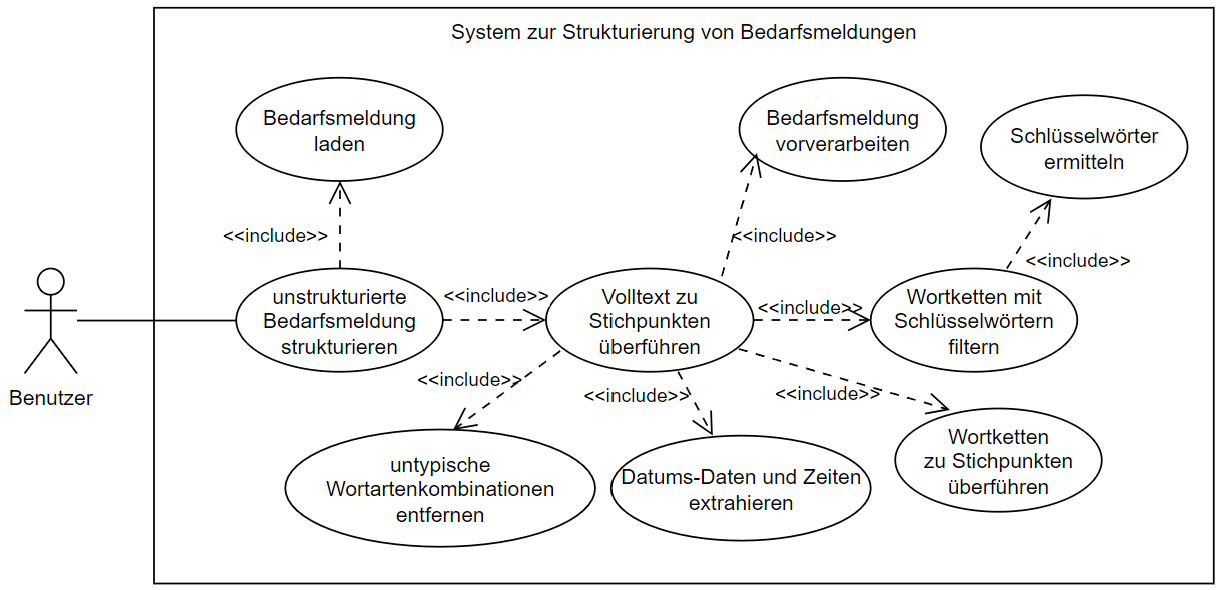
\includegraphics[width=\linewidth]{Abbildungen/use-case.png}
	\caption{Use-Case Diagramm zum System zur Strukturierung von Bedarfsmeldungen.}
	\label{fig:usecasediagrammwirklich}
\end{figure}\mbox{} \\
In der Abbildung \ref{fig:usecasediagrammwirklich} ist das Use-Case Diagramm zum System zur Strukturierung von \emph{Bedarfsmeldungen} dargestellt. Es existiert ein Akteur, der die Bezeichnung \emph{Benutzer} hat. Dieser hat die Möglichkeit unstrukturierte \emph{Bedarfsmeldungen} zu strukturieren. Dazu kann das System einerseits eine \emph{Bedarfsmeldung} laden und im Falle der unstrukturierten Volltexfelder eine Reihe an Aufgaben durchführen. Um die Volltexte in Stichpunkte zu überführen, kann der Text mit Vorverarbeitungsverfahren reduziert und angepasst werden. Im Rahmen der Überführung von Stichpunkten können die aus den Volltext erstellten Wortketten auf die gekürzt werden, die mindestens ein Schlüsselwort enthalten. Die Schlüsselwörter können zudem ermittelt werden. Im Anwendungsfall der Überführung des Volltextes in Stichpunkte, können Wortartkombinationen, die nicht zusammengehören in den Wortketten entfernt werden. Dadurch trennen sich neben der Filterung von Schlüsselwörter weitere Verbindungen innerhalb der Wortketten. Datums- und Zeitangaben können neben den anderen Anwendungsfällen separat herausgefiltert werden. Schließlich können die Wortketten zu Stichpunkten überführt werden.
%Dieser hat die Möglichkeit eine oder mehrere \emph{Bedarfsmeldungen} zu laden. Zudem kann diese ins Englische übersetzt werden. Darüber hinaus kann die \emph{Bedarfsmeldung} durch \emph{Preprocessing} vorverarbeitet werden und irrelevante Wörter und Zeichen aus der \emph{Bedarfsmeldung} ausschließen. Der Benutzer kann die Methoden \emph{TF-IDF}, \emph{TextRank}, \emph{N-Gram}, \emph{POS-Tagging} und \emph{NER} mit der \emph{Bedarfsmeldung} anwenden. Wenn mehrere Methoden in der Pipeline sind, können die Resultate durch die Anwendung von \emph{Data-Fusion} zusammengeführt werden.
\subsection{Anforderungen}
Im Folgenden werden die funktionalen sowie nichtfunktionalen Anforderungen des Systems beschrieben. Diese Informationen wurden aus den Ergebnissen des Kapitels \ref{chap:erwartungshaltung} und dem Kapitel \ref{sec:anforderungsanalyse} hergeleitet und bilden den Rahmen des Systems.
\subsubsection{Funktionale Anforderungen}
Die funktionalen Anforderungen beschreiben konkrete Funktionalitäten des Systems. Dazu werden zusammengehörende Anforderungen nummeriert und in detaillierte Unterpunkte aufgelistet und beschrieben.
\begin{enumerate}[label=1.\arabic*]
	\item Die \emph{Bedarfsmeldungen} sollen geladen werden können.
	\item Beim laden wird eine \emph{Bedarfsmeldung} ausgewählt.
	\item Die ausgewählte \emph{Bedarfsmeldung} muss in die vordefinierte Struktur überführt werden.
\end{enumerate}
\begin{enumerate}[label=2.\arabic*]
	\item Das System soll Methoden der Vorverarbeitung zur Bereinigung eines Volltextes anwenden können.
	\item Die Vorverarbeitung soll ein Volltext als Eingabe erhalten.
	\item Das Vorverarbeitung soll den bereinigten Volltext als Ausgabe zurückgeben.
\end{enumerate}
\begin{enumerate}[label=3.\arabic*]
	\item Das System soll eine Methode zur Identifizierung von Schlüsselwörtern anwenden können.
	\item Das Modul soll eine Liste mit Schlüsselwörtern anlegen.
\end{enumerate}
\begin{enumerate}[label=4.\arabic*]
	\item Das System soll Wortketten aus einem Volltext erstellen können.
	\item Das Modul soll einen Volltext als Eingabe für diese Methode erhalten.
	\item Als Rückgabe soll das Modul eine Liste mit Wortketten zurückgeben.
	\item Das System soll eine Wortketten-Liste auf die Wörter reduzieren, die mindestens ein Schlüsselwort enthalten.
\end{enumerate}
\begin{enumerate}[label=5.\arabic*]
	\item Das System soll eine Methode zur Extraktion von Zeitangaben anwenden können.
	\item Das Modul soll aus einem Volltext Datums- und Zeitangaben extrahieren.
\end{enumerate}
\begin{enumerate}[label=6.\arabic*]
	\item Das System soll eine Methode zur Identifikation von untypischenn Wortkombinationen anwenden können.
	\item Das Modul soll Wortkombinationen aus der Wortkette erhalten und überprüfen ob die Wörter nebeneinander stehen dürfen.
	\item Wortketten werden entfernt, die nicht nebeneinander stehen sollen.
\end{enumerate}
\begin{enumerate}[label=7.\arabic*]
	\item Das System soll die Wortketten in zusammengehörende Stichpunkte zusammenführen.
	\item Als Ergebnis wird eine Liste mit Stichpunkten zurückgegeben.
\end{enumerate}
\begin{enumerate}[label=8.\arabic*]
	\item Die in Stichpunkte umgebauten Volltexte werden der \emph{Bedarfsmeldung} beigefügt.
	\item Die Datums- und Zeitangaben werden den Stichpunkten beigefügt.
	\item Das Ergebnis wird dem Benutzer ausgegeben.
\end{enumerate}
\subsubsection{Nichtfunktionale Anforderungen}
Hierbei handelt es sich um qualitätsbezogene Anforderungen. Diese umfassen nicht konkrete Funktionen des Systems, sondern stellen Rahmenbedingungen des Systems im Ganzen zusammen.
\begin{enumerate}
	\item Das System soll modular aufgebaut sein, um die einzelnen Schritte und Methoden austauschen zu können.
	\item Das System soll in der Lage sein, mehrere \emph{Bedarfsmeldungen} laden zu können.
	\item Das System muss in der Lage sein, die \emph{Bedarfsmeldungen} in einer akzeptablen Zeitspanne zu verarbeiten.
	\item Das Ergebnis muss deterministisch sein.
\end{enumerate}
\subsection{Ablauf des Systems}
Der Ablauf des Systems zur Strukturierung von \emph{Bedarfsmeldungen} wird mit Hilfe eines UML-Aktivitätsdiagramm dargestellt, das eine Erweiterung des Aktivitätsdiagramms aus der Abbildung \ref{fig:recommendersystem} durch eine hierarchische Schachtelung darstellt.
\begin{figure}[H]
	\centering  
	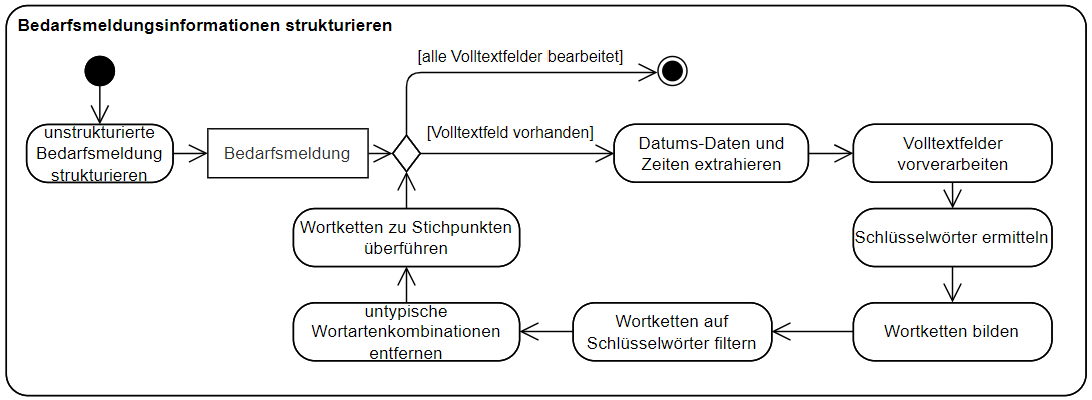
\includegraphics[width=\linewidth]{Abbildungen/bedarfsmeldungstrukturieren.png}
	\caption{Abstrakte Darstellung des Systems zur Strukturierung von \emph{Bedarfsmeldungen}.}
	\label{fig:ablaufsystemabstrakt}
\end{figure}\mbox{} \\
In Abbildung \ref{fig:ablaufsystemabstrakt} ist der abstrakte Ablauf des Systems dargestellt. Zu Beginn wird der unstrukturierte Informationsfelder mit \emph{Bedarfsmeldungsinformationen} in eine strukturierte Form gebracht. Anschließend werden die Volltextfelder durch eine Reihe an Schritten geleitet. Angefangen mit der Extraktion von Datums-Daten und Zeiten. Die Volltextfelder werden vorverarbeitet, wodurch ungewollte Formatierungen entfernt werden. Darauffolgend werden Schlüsselwörter im Volltext ermittelt. Aus dem Volltext werden Wortketten gebildet und auf die Wörter reduziert, die Schlüsselwörter enthalten. Dann werden untypische Wortartenkombinationen entfernt, wodurch die Wortketten weiter separiert werden. Zum Schluss werden die einzelnen Wortketten in Stichpunkte überführt und in die \emph{Bedarfsmeldung} aufgenommen. Dieser Prozess wird für alle Volltextfelder durchgeführt.